% beamer
\documentclass{clsemhs11-beamer}
\usepackage[ngerman]{babel}
\usepackage[utf8]{inputenc}
\usepackage[T1]{fontenc}
\usepackage{helvet}
\usepackage{beamerthemesplit}
\usepackage[numbers]{natbib}

\newcommand{\first}[1]{\emph{#1}}
\newcommand{\q}[1]{\iflanguage{ngerman}{\flqq#1\frqq}{``#1''}}

\title{Open Source-MÜ-Systeme}
\subtitle{Seminar \q{Maschinelle \"Ubersetzung} (HS~2011)}
\author{Simon Hafner \& Hernani Marques}
\date{\today}

\begin{document}
  \maketitle


\begin{frame}
\frametitle{Referatsübersicht}
\tableofcontents
\end{frame}

%%%%%%%%%%%%%%%%%%%%%%%%%%%%%%%%%%%%%%%%%%%%%%%%%%%%%%%%%%%%%%%%%%%%%%%%%%%%%
% SECTION
%%%%%%%%%%%%%%%%%%%%%%%%%%%%%%%%%%%%%%%%%%%%%%%%%%%%%%%%%%%%%%%%%%%%%%%%%%%%%
\section{Problemstellung}
\subsection{Warum Closed Source vs. Open Source Software?}
\begin{frame}
\frametitle{Open Source Software}
\begin{figure}
  
\includegraphics[width=0.35\textwidth]{graphics/ossmatrix}
  \caption{Open Source Software (Logos)\footnote{URL: \url{http://cdn.lostintechnology.com/wp-content/uploads/2010/12/opensource.jpg} (29.11.2011)}}
  \end{figure}
\end{frame}
\subsection{Minderheitensprachen}
%%%%%%%%%%%%%%%%%%%%%%%%%%%%%%%%%%%%%%%%%%%%%%%%%%%%%%%%%%%%%%%%%%%%%%%%%%%%%
% SECTION
%%%%%%%%%%%%%%%%%%%%%%%%%%%%%%%%%%%%%%%%%%%%%%%%%%%%%%%%%%%%%%%%%%%%%%%%%%%%%
\section{Herausforderungen \& Lösungsansätze}
\subsection{Sparse data-Probleme}
%%%%%%%%%%%%%%%%%%%%%%%%%%%%%%%%%%%%%%%%%%%%%%%%%%%%%%%%%%%%%%%%%%%%%%%%%%%%%
% SECTION
%%%%%%%%%%%%%%%%%%%%%%%%%%%%%%%%%%%%%%%%%%%%%%%%%%%%%%%%%%%%%%%%%%%%%%%%%%%%%
\section{Zwei OSS-MÜ-Systeme: Apertium und Moses}
\subsection{Apertium}
\subsection{Moses}
%%%%%%%%%%%%%%%%%%%%%%%%%%%%%%%%%%%%%%%%%%%%%%%%%%%%%%%%%%%%%%%%%%%%%%%%%%%%%
% SECTION
%%%%%%%%%%%%%%%%%%%%%%%%%%%%%%%%%%%%%%%%%%%%%%%%%%%%%%%%%%%%%%%%%%%%%%%%%%%%%
\section{Literatur}
\begin{frame}
  \frametitle{Lektüreempfehlungen}

\begin{thebibliography}{...............}
\bibitem[Norvig1992]{norvig}
Norvig, Peter: \emph{Paradigms of artificial intelligence programming: case studies in common LISP}. S.195-196. San Fransisco: Morgan.
\bibitem[Forcada2010]{forcadaDoc}
Forcada Mikel L. et al.: \emph{Documentation of the Open-Source Shallow-Transfer Machine Translation Platform Apertium}.\\
URL: \url{http://xixona.dlsi.ua.es/~fran/apertium2-documentation.pdf} (29.11.2011)

\bibitem[Forcada2006]{forcada}
Forcada, Mikel L.: \emph{Open-source machine translation: an opportunity for minor languages}. In: Strategies for developing machine translation for minority languages (5th SALTMIL workshop on Minority Languages).\\URL: \url{http://www.dlsi.ua.es/~mlf/docum/forcada06p2.pdf} (29.11.2011)
\end{thebibliography}

\end{frame}
%%%%%%%%%%%%%%%%%%%%%%%%%%%%%%%%%%%%%%%%%%%%%%%%%%%%%%%%%%%%%%%%%%%%%%%%%%%%%
% SECTION
%%%%%%%%%%%%%%%%%%%%%%%%%%%%%%%%%%%%%%%%%%%%%%%%%%%%%%%%%%%%%%%%%%%%%%%%%%%%%
\section{Fragen}
\begin{frame}
  \begin{figure}
  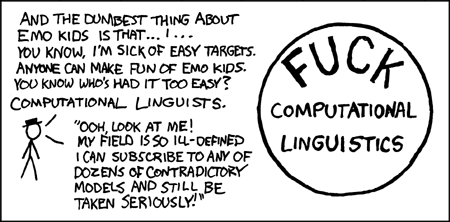
\includegraphics[width=0.35\textwidth]{graphics/xkcd--cl}
  \caption{XKCD - Nr. 114\footnote{URL: \url{http://xkcd.com/114/} (29.11.2011)}}
  \end{figure}
\end{frame}
\end{document}
